\documentclass{article}
\usepackage{amsfonts}
\usepackage{amsmath}
\usepackage{amsthm}
\usepackage{graphicx}
\usepackage[letterpaper, margin=.75in]{geometry}
\usepackage{multicol}
\usepackage{graphpap}
%\usepackage{pdfpages}
%\usepackage{enumerate}
\usepackage[shortlabels]{enumitem}
\usepackage{tabularx}
\usepackage{framed}
\usepackage{tikz}
\usepackage{pgfplots}
% \usepackage{tcolorobox}

\usetikzlibrary{arrows, calc, patterns, positioning, shapes}
\newcommand{\degree}{$^{\circ}$}
\newcounter{probno}[enumi]
\newcommand{\hitem}{\hfill \stepcounter{probno} (\roman{probno})\hspace{1em}}
\newenvironment{hnumerate}{\begin{center}}{\hfill\setcounter{probno}{0}\end{center}}
\pgfplotsset{compat=1.9}

% change hyperref options
\PassOptionsToPackage{hyphens}{url}
\usepackage[bookmarks,colorlinks,linkcolor=blue,citecolor=blue,pdfstartview=FitH,urlcolor=blue]{hyperref}

\newcounter{currentyear}
\setcounter{currentyear}{2023}

\newcounter{eqnno}[enumi]
\newcommand{\eqn}{\stepcounter{eqnno} (\theeqnno) \label{05table\theeqnno}}

\newenvironment{teacher}[1]{\begin{center}
	\textbf{#1}
\end{center}\vspace{-3ex}\begin{framed}}{\end{framed}}

\newcommand{\goals}[1]{
\fbox{
\parbox{\textwidth}{
  \textbf{\textsf{ \large Student learning objectives:}}
    #1
}
}
  % \begin{tcolorbox}[colframe=purple, colback=purple!10!white]

  % \end{tcolorbox}
  }

\newif\ifteacher
\pagestyle{empty}
\setcounter{secnumdepth}{0}
 \newcounter{saveenumi}
 \newcounter{saveenumi1}
\newtheorem{qkrev}{Quick Review Question}
 
\setcounter{saveenumi}{0}
\newenvironment{countme}{\begin{enumerate} \setcounter{enumi}{\thesaveenumi}}{\setcounter{saveenumi}{\theenumi} \end{enumerate}}
\newenvironment{multic}[1]{\begin{multicols}{#1}\begin{countme}}{\end{countme}\end{multicols}}

\newcounter{sectno} \newcounter{chaptno}
\newcommand{\question}[1]{\noindent \textbf{#1 Point Question:} \\}
\newcommand{\worksheet}[1]{\Large \textbf{Chapter \thechaptno}  \hfill  IS 101 \section{#1} \par \normalsize}
%\newcommand{\vensim}{\emph{Vensim} \textsuperscript{\textregistered} PLE }

\newcommand*\cleartooddpage{%
  \clearpage%
  \ifodd\value{page} \else\thispagestyle{empty}\begin{center}\em This page intentionally left blank.\end{center}\clearpage\fi}

\includeonly{
%Curry,
%DiMaggio,
%Uconn,
%Unbreakable,
%NFLPlayoff,
%FIFA,
%Fridge,
%Morgan,
%Tiger,
Moneyball,
}


\begin{document}
\setcounter{chaptno}{2}
\worksheet{Shoot 3's like Steph Curry}
Things you will need"'
\begin{itemize}
	\item coin
	\item this worksheet
\end{itemize}

We're ready to play our game. Curry's results are locked in; he's made 11 of 13 three-point attempts. Now you need to take your 13 shots.
\vfill

\begin{enumerate}
	\item Flip a coin
	\item If you get heads, you make the shot; tails, you miss.
	\item Repeat the coin flip 13 times and keep track of your progress with the chart below. \vfill
	
	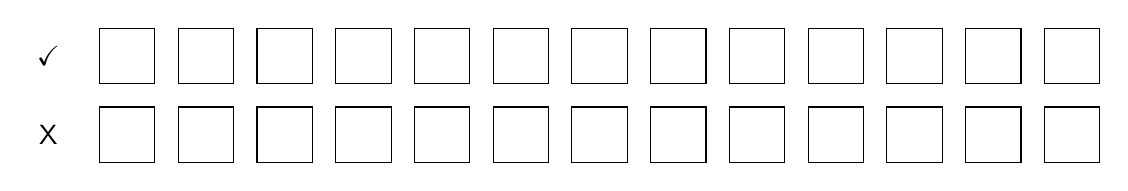
\begin{tikzpicture}
	\node at (0,0) {$\checkmark$};
		 \foreach \x in {1,...,13}{
       \node [inner sep=10pt, draw] at  (\x,0)  {};
       }
	\node at (0, -1) {\sffamily X};
		 \foreach \x in {1,...,13}{
       \node [inner sep=10pt, draw] at  (\x,-1)  {};
       }
	\end{tikzpicture}
\end{enumerate}

Did you beat Steph by making more than 11 shots? If so, you are lucky. Play a couple more games:\vfill
	
	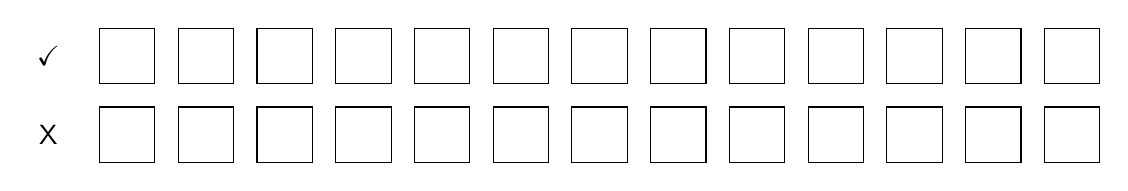
\begin{tikzpicture}
	\node at (0,0) {$\checkmark$};
		 \foreach \x in {1,...,13}{
       \node [inner sep=10pt, draw] at  (\x,0)  {};
       }
	\node at (0, -1) {\sffamily X};
		 \foreach \x in {1,...,13}{
       \node [inner sep=10pt, draw] at  (\x,-1)  {};
       }
	\end{tikzpicture}\vfill
	
	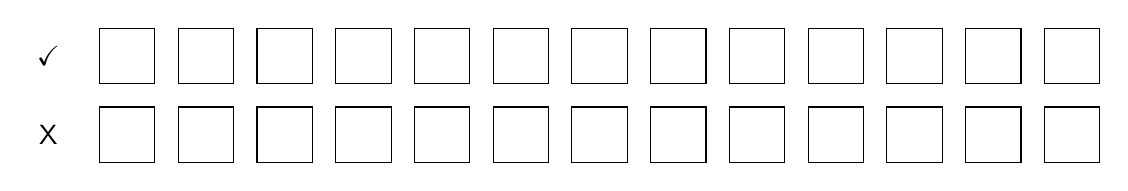
\begin{tikzpicture}
	\node at (0,0) {$\checkmark$};
		 \foreach \x in {1,...,13}{
       \node [inner sep=10pt, draw] at  (\x,0)  {};
       }
	\node at (0, -1) {\sffamily X};
		 \foreach \x in {1,...,13}{
       \node [inner sep=10pt, draw] at  (\x,-1)  {};
       }
	\end{tikzpicture}\vfill
	
	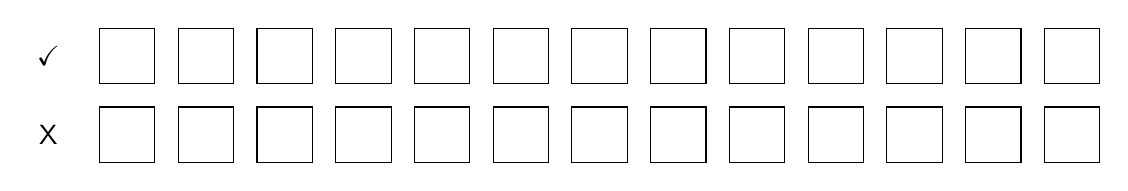
\begin{tikzpicture}
	\node at (0,0) {$\checkmark$};
		 \foreach \x in {1,...,13}{
       \node [inner sep=10pt, draw] at  (\x,0)  {};
       }
	\node at (0, -1) {\sffamily X};
		 \foreach \x in {1,...,13}{
       \node [inner sep=10pt, draw] at  (\x,-1)  {};
       }
	\end{tikzpicture}\vfill
	
	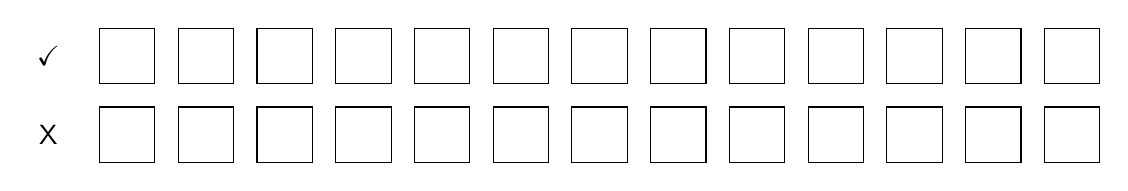
\begin{tikzpicture}
	\node at (0,0) {$\checkmark$};
		 \foreach \x in {1,...,13}{
       \node [inner sep=10pt, draw] at  (\x,0)  {};
       }
	\node at (0, -1) {\sffamily X};
		 \foreach \x in {1,...,13}{
       \node [inner sep=10pt, draw] at  (\x,-1)  {};
       }
	\end{tikzpicture}
	
	What is the average number of three point shots you are making in each game?


\stepcounter{chaptno}
\worksheet{Dicey Hitting Streak}


\begin{enumerate}
\subsection{Did it happen or not?}
	\item If the probability that something happens is $1/4$, why is the probability that it doesn't happen $1-1/4$? \vfill
	
	\item If the probability that something happens is $p$, what is the probability that it doesn't happen? \vfill
	
	\subsection{Oddly Enough}
	\item It is common for people to talk about probabilities with the language of odds. So, something that happens $1/4$ of the time has odds of about one in four.  If you have a probability $p$, you can write down the odd by just letting the second number be $1/p$.
	
	\item If the probability that something happens is $0.001$, what are the odds that it happened? \vfill
	
\subsection{Did it happen a lot?}
	
	\item If the probability that you roll a 1 with your dice is $\frac{1}{6}$, why is the probability that you roll a 1 twice with two rolls $(\frac{1}{6})^2$? \vfill
	
	\item If the probability that something happens is $p$, what is the probability that it happens twice in two tries?
	
\subsection{Combine the ideas}

	\item What is the probability that you roll a dice three times and only get one ``1''? \vfill
	
	\item What is the probability that you and your partner don't have the same birthday? Hint: Assume there are 365 days in a year. \vfill
	
	\item What is the probability that no one in the room has the same birthday? \vfill
	
	\clearpage
	\subsection{Hitting Streak}
	\item Joe DiMaggio got a hit in 56 straight games.
\begin{enumerate}
	\item Roll a die.
	\item If you get a 6, you end the game hitless and Joe wins the contest. Else, you get a hit in one game.
	\item Keep track of your progress with the chart below, through 56 games or until your streak ends.
\end{enumerate}
\begin{center}
		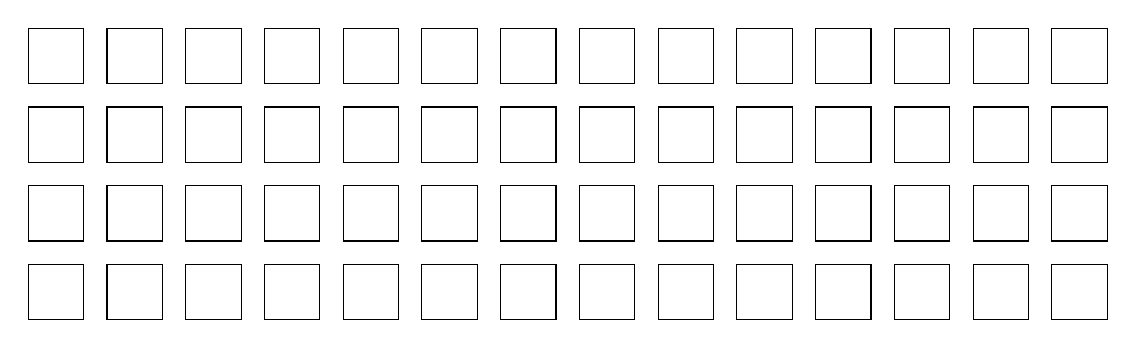
\begin{tikzpicture}
	%\node at (0,0) {$\checkmark$};
		 \foreach \x in {1,...,14}{
		\foreach \y in {0,...,3}{
       \node [inner sep=10pt, draw] at  (\x,\y)  {};
       }
			}
	\end{tikzpicture}
\end{center}

\item What is the probability that you match Joe's streak?  What are the odds of that happening?
\end{enumerate}
\stepcounter{chaptno}
\worksheet{Racking Up The Wins}
\begin{enumerate}
	\item The UConn women's basketball team won 111 straight games. How many can you win?
\begin{enumerate}
	\item Calculate the probability that if you roll three dice, you don't get three ones. \vfill
	\item Roll three dice (or one dice three times) to see if you win or lose a game.  If you don't want to actually roll the dice, you can open up a browser and type ``roll dice'' into Google, then click the square two more times to get three six-sided dice to roll. 
	\item If you get three ones, you lose the game; else you win.
	\item Repeat this until you lose a game or win 111 games. Tally your winning streak with the chart below.
	
	\begin{center}
		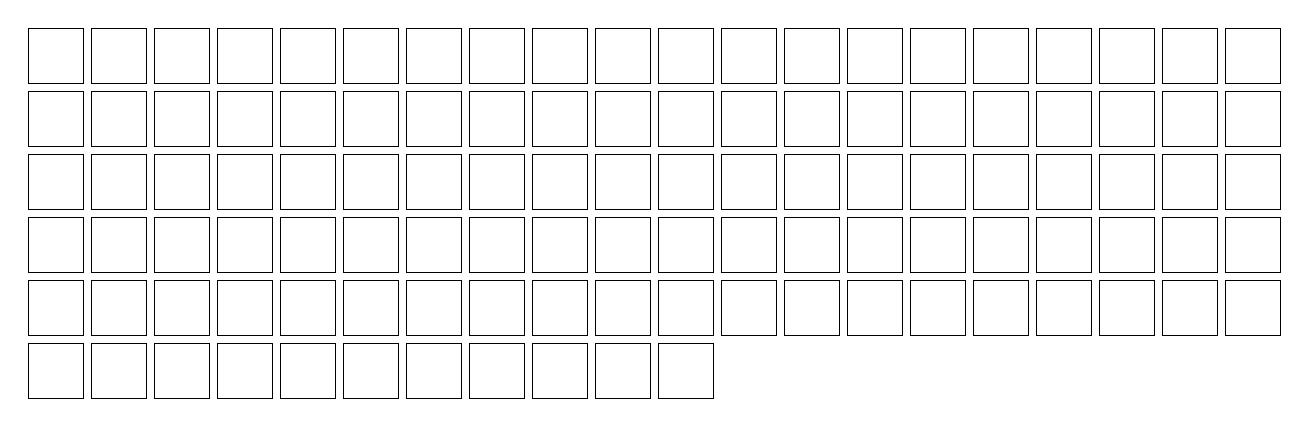
\begin{tikzpicture}[scale=.8]
		\foreach \x in {1,...,11}{
       \node [inner sep=10pt, draw] at  (\x,0)  {};
			}
		 \foreach \x in {1,...,20}{
		\foreach \y in {1,...,5}{
       \node [inner sep=10pt, draw] at  (\x,\y)  {};
       }
			}
	\end{tikzpicture}
	\end{center}
	\vfill
\end{enumerate}
\item What is a factorial and what is the formula for \(10!\)?\vfill
\clearpage
\item What is a permutation? What is the formula for \(P(8,3)\)? If there are 8 Varsity Cross-Country runners, how many ways can they take first, second, and third place in one race? \vfill
\item What is a combination? What is the formula for \(C(9,4)\)? How many ways can Wartburg Men's Soccer team tie 4 of their first 9 games ? \vfill
\item What is the formula for the probability of \(r\) successes out of \(n\) attempts where the probability of each success is \(p\)? Georgia Nissen has an overall tennis singles record of 4-2, use that record to calculate the probability that she wins 3 of her next 4 games? \vfill
\end{enumerate}
\stepcounter{chaptno}
\worksheet{Unbreakable Tennis}
The first player to win four or more points and be ahead by two points wins the \textbf{game}. In tennis, the score begins at ``love,'' or zero points. Wining a point takes a player to 15, then 30, then 40, and then game point, which wins the game unless the players are tied 40-40, which is called a ``deuce,'' From deuce, the game proceeds until a player pulls ahead by two points.
\begin{enumerate}
	\item Serve like Agassi
	\begin{itemize}
		\item First serve: flip a coin three times.
		\begin{itemize}
			\item If exactly two tails, serve is out. Go to second serve.
			\item Else, serve is in. Play proceeds: flip a coin two times.
			\begin{itemize}
				\item If exactly two tails, Agassi loses the point.
				\item Else, Agassi winds the point.
			\end{itemize}
			\item Second serve: flip a coin one time.
			\begin{itemize}
				\item If tails, Agassi loses the point.
				\item If heads, Agassi wins the point.
			\end{itemize}
		\end{itemize}
	\end{itemize}
	Practice playing as Agassi.
	
	\begin{tabular}{*{13}{c}}
	Game  & Initials&\\
	\hline
	1 & & S: & 15 & 30 & 40 & S &S &S &S &S &S &S\\
	&&    R: & 15 & 30 & 40 & R &R &R &R &R &R &R\\ \hline
	%2 & & S: & 15 & 30 & 40 & S &S &S &S &S &S &S\\
	%&&    R: & 15 & 30 & 40 & R &R &R &R &R &R &R\\ \hline
	%3 & & S: & 15 & 30 & 40 & S &S &S &S &S &S &S\\
	%&&    R: & 15 & 30 & 40 & R &R &R &R &R &R &R\\ \hline
	%4 & & S: & 15 & 30 & 40 & S &S &S &S &S &S &S\\
	%&&    R: & 15 & 30 & 40 & R &R &R &R &R &R &R\\ \hline
	%5 & & S: & 15 & 30 & 40 & S &S &S &S &S &S &S\\
	%&&    R: & 15 & 30 & 40 & R &R &R &R &R &R &R\\ \hline
	%6 & & S: & 15 & 30 & 40 & S &S &S &S &S &S &S\\
	%&&    R: & 15 & 30 & 40 & R &R &R &R &R &R &R\\ \hline
	\end{tabular}
	
	\item Play like Sampras
	\begin{itemize}
		\item You can ask the computer to calculate a random number between 0 and 1 by typing \texttt{= RAND()} into either Excel or Google Sheets.
		\item Pick a random number between 0 and 1. If the number is less than 0.5947, Samparas's first serve goes in.
		\item If the first serve goes in, pick another uniform random number between 0 and 1. It it is less than 0.8092, then Sampras wins the point.
		\item If the first serve didn't go in, pick a uniform random number between 0 and 1 for the second serve, and if it is less than 0.5261, then Sampras wins the point.
	\end{itemize}
	Practice playing as Sampras for one game:
	
	\begin{tabular}{*{13}{c}}
	Game  & Initials&\\
	\hline
	1 & & S: & 15 & 30 & 40 & S &S &S &S &S &S &S\\
	&&    R: & 15 & 30 & 40 & R &R &R &R &R &R &R\\ \hline\end{tabular}
	
	\clearpage
	\item Now have them play each other:
	
	\begin{tabular}{*{13}{c}}
	Game  & Initials&\\
	\hline
	1 & & S: & 15 & 30 & 40 & S &S &S &S &S &S &S\\
	&&    R: & 15 & 30 & 40 & R &R &R &R &R &R &R\\ \hline
	2 & & S: & 15 & 30 & 40 & S &S &S &S &S &S &S\\
	&&    R: & 15 & 30 & 40 & R &R &R &R &R &R &R\\ \hline
	3 & & S: & 15 & 30 & 40 & S &S &S &S &S &S &S\\
	&&    R: & 15 & 30 & 40 & R &R &R &R &R &R &R\\ \hline
	4 & & S: & 15 & 30 & 40 & S &S &S &S &S &S &S\\
	&&    R: & 15 & 30 & 40 & R &R &R &R &R &R &R\\ \hline
	5 & & S: & 15 & 30 & 40 & S &S &S &S &S &S &S\\
	&&    R: & 15 & 30 & 40 & R &R &R &R &R &R &R\\ \hline
	6 & & S: & 15 & 30 & 40 & S &S &S &S &S &S &S\\
	&&    R: & 15 & 30 & 40 & R &R &R &R &R &R &R\\ \hline
	\end{tabular}
	
	\item Calculate the probability of a set reaching a 6-6 tie with neither player losing serve:
	\begin{itemize}
		\item The probability that Sampras wins one straight service game is 0.89. What is the probability that he wins 6 straight service games? \underline{\vspace{1in}}
		\item The probability that Agnassi wins one straight service game is 0.84. What is the probability that he wins 6 straight service games? \underline{\vspace{1in}}
		\item The probability that they reach 6-6 is the product of your two answers:  \underline{\vspace{1in}} What is the probability that they play four sets with neither player losing serve?  \underline{\vspace{1in}}
	\end{itemize}
\end{enumerate}
\stepcounter{chaptno}
\worksheet{NFL Drive}

Roll a die four times to determine the outcome of your NFL possession:

\begin{itemize}
	\item Safety -- if you roll four 2's, four 3's, four 4's, or four 5's, giving a probability of 4/1296 = 0.003
	\item Touchdown -- if you roll
	\begin{itemize}
		\item 1 on the first roll, giving \(6^3=216\) options or 
		\item 2-3 or 3-4 on the fist two rolls giving an additional \(2\times 6^2\) 
	\end{itemize}
	\item Field goal -- if you roll 6 on the first roll, giving a probability of \(6^3/6^4 = 0.17\).
	
	\hline
	When you score a touchdown you get 6 points. Determine if you add 0, 1, or 2 additional points by rolling a die twice. Note that the two-point conversions are attempted after a touchdown \(113/(113+1210)\), or 8.5\% of the time.
	\item If you roll 1-1, 2-2, or 3-3, you are attempting a two-point conversion, which equates to a probability of \((3\times6^2)/6^4\), or 8.3\%. Roll one die a third time, and if you get  1, 2, 3 you score 2 points, which occurs 50\% of the time.
	\item Otherwise (if you didn't roll 1-1, 2-2, or 3-3) you are attempting an extra point. Roll one die two more times. If you roll anything but 1-1, or 2-2, you score 1 point, which occurs with a probability equal to \(1-(2\times 6^2)/6^4 = 0.944\).
\end{itemize}

\stepcounter{chaptno}
\worksheet{FIFA Octopus Oracle}

\textbf{Paul the Octopus's Predictions}

Let's make FIFA predations by guessing,

\begin{enumerate}
	\item Flip a coin 14 times.
	\item Keep track of the number of heads and tails in the grid below.
	\item You match Paul's unlikeliness by getting heads 2 or 12 times.
	\item You beat Paul's unlikeliness by getting heads 0, 1, 13, or 14 times.
	
		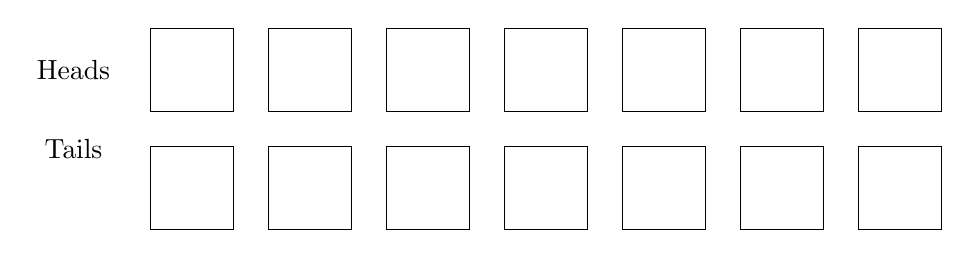
\begin{tikzpicture}
	\node at (0,0) {Heads};
		 \foreach \x in {1,...,7}{
       \node [inner sep=15pt, draw] at  (1.5*\x,0)  {};
       }
	\node at (0, -1) {Tails};
		 \foreach \x in {1,...,7}{
       \node [inner sep=15pt, draw] at  (1.5*\x,-1.5)  {};
       }
	\end{tikzpicture}
	
\noindent\rule[0.5ex]{\linewidth}{1pt}
	
		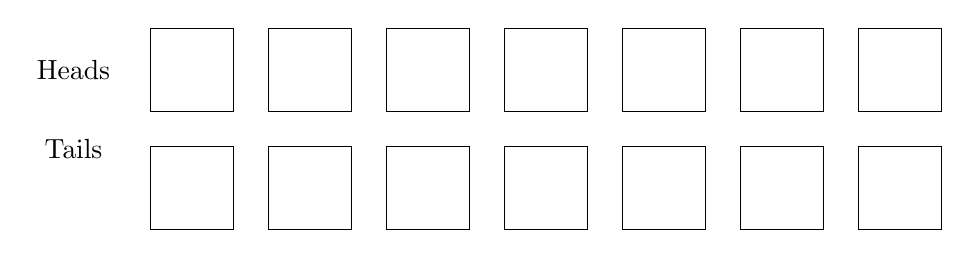
\begin{tikzpicture}
	\node at (0,0) {Heads};
		 \foreach \x in {1,...,7}{
       \node [inner sep=15pt, draw] at  (1.5*\x,0)  {};
       }
	\node at (0, -1) {Tails};
		 \foreach \x in {1,...,7}{
       \node [inner sep=15pt, draw] at  (1.5*\x,-1.5)  {};
       }
	\end{tikzpicture}
	
	Just as before, it is quicker to use the Bernoulli formula to calculate these probabilities exactly:
	\[ \text{The probability of \(r\) successes out of \(n\) attempts where the probability of each success is \(p\) } = C(n,r)\times p^r \times p^{n-r}\] 
	\item Calculate the probability that you match Paul's unlikeliness using the Bernoulli formula.
	\vfill
		\item Calculate the probability that you beat Paul's unlikeliness using the Bernoulli formula.
	\vfill
	
	\item In statistics, as a rule of thumb, we say that something is rare if the probability that it happens is less than 5\%. Which of the two outcomes could we call rare? Do you agree? \vfill
\end{enumerate}
\stepcounter{chaptno}
\worksheet{Super-Sized Super Bowl}

\textbf{Weight and NFL Defensive Tackles}

Each roll simulates pulling a random player who has played defensive line or defensive tackle in the NFL.
\begin{enumerate}
	\item Roll two dice (or one die twice)
	\item If you roll a 12 (two 6's), then your player weighs at least 325 pounds.
	\item Else, your player weighs less than the Fridge.
\end{enumerate}

Try it several times. Did you get anyone heavier than Perry? If so, how many?\vfill

\textbf{Two Point Conversions}

In the NFL, after a touch-down is scored, the team has the choice of kicking the ball through the goal posts for one extra point or physically getting the ball to an offensive player in the end zone for two extra points. Which choice the coach makes depends on a lot of different factors including the skill of their players, but the main decision factor is often the difference in points that the team has compared to their opponent.

\begin{enumerate}
	\item \textbf{Game Situation 1: Team A trailing by 8 points (16-24) with 5 minutes left in the 4th quarter.}
After scoring a touchdown, what should Team A's coach call?

Probabilities: 
\begin{itemize}
	\item Probability of successfully converting a two-point conversion: 45%
	\item Probability of successfully converting an extra point kick: 95%
	\item Probability of stopping the opponent and getting another possession: 30% 
\end{itemize}
Calculate the expected points gained by attempting a two-point conversion versus an extra point kick and the probability of winning the game based on these numbers.  

What are some additional complications that you would want to build into the decision-making analytics if you had more time?
\vfill

\item Game Situation 2: Team B leading by 6 points (21-15) with 2 minutes left in the 4th quarter.
After scoring a touchdown, what should Team B's coach call?

Probabilities:
\begin{itemize}
	\item Probability of successfully converting a two-point conversion: 50%
	\item Probability of successfully converting an extra point kick: 97%
	\item Probability of stopping the opponent and getting another possession: 40%
\end{itemize}

Determine whether attempting a two-point conversion in this situation is the right call for Team B. 

What are some additional complications that you would want to build into the decision-making analytics if you had more time?\vfill

\end{enumerate}


\stepcounter{chaptno}
\worksheet{Scoring Confidence}

\textbf{Scoring Like Alex Morgan}
See if you score a goal in a cap:
\begin{enumerate}
	\item Roll a die.
	\item If you roll a 1, 2, 3, or 4, you score; else you don't.	
	\item Repeat this ten times and keep track of your progress with the chart below.
\end{enumerate}
\begin{center}
		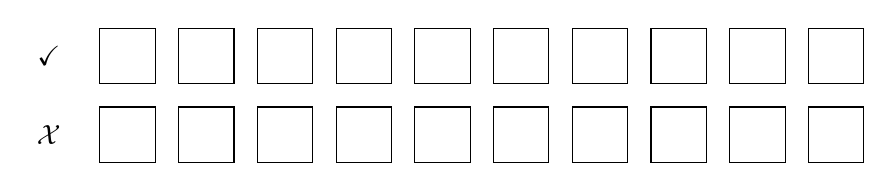
\begin{tikzpicture}
	\node at (0,1) {$\checkmark$};
	\node at (0,0) {$\mathcal{X}$};
		 \foreach \x in {1,...,10}{
		\foreach \y in {0,...,1}{
       \node [inner sep=10pt, draw] at  (\x,\y)  {};
       }
			}
	\end{tikzpicture}
\end{center}
\vfill
\textbf{Creating a Program}
\begin{itemize}
	\item For each game, pick a uniform random number between 0 and 1.
	\item If the number is less than 0.629, Morgan scores in the game. Else, she doesn't.
	\item Play 159 games, tally the number of games in which she scores, and compute the goals/cap rate.
	\item Repeat ten thousand times.
\end{itemize}

\begin{itemize}
	\item What simplifying assumptions are we making in our program?\vfill
	\item What would you change in the program if you were running a simulation for Mia Hamm? \vfill
\end{itemize}


\stepcounter{chaptno}
\worksheet{Tiger's Consistency}

To model a round of golf, roll two dice You score 70 with a roll that sums to 7. A sum of 6 corresponds to scoring one stroke below 70 (69), and a sum of 8, one stroke above (71). Foe each number below a sum of 6, we'll subtract two additional strokes, and for each number above a sum of 8, we'll add two strokes.
\begin{enumerate}
	\item Is it possible to score a 74 using this simulation? Why or why not? \vfill
	\item Fill in the table for the dice roll model:
	
	\begin{center} \Large
		\begin{tabular}{c|c}
		Dice Roll & Round Score\\\hline
		4 & \\\hline
		5 & \\\hline
		6 & 69\\\hline
		7 & 70\\\hline
		8 & 71\\\hline
		9 & \\\hline
		10 & \\\hline
		\end{tabular}
	\end{center}\normalsize
	
	\item How well does the model fit the statement ``In the PGA, the average first round score is about 70 with a standard deviation of about 4.''
	\begin{enumerate}
		\item What scores would be included in the statement ``within one standard deviation of the mean''?\vfill
		\item What percentage of the rounds should be within one standard deviation of the mean? \label{tiger1}\vfill
		\item How many different dice rolls will give you scores within one standard deviation of the mean? \label{tiger2}
		\begin{center} \large
			\begin{tabular}{c*{6}{|c}}
			 & 1 & 2 & 3 & 4 & 5 & 6\\\hline
			1&&&&&&\\\hline
			2&&&&&&\\\hline
			3&&&&&&\\\hline
			4&&&&&&\\\hline
			5&&&&&&\\\hline
			6&&&&&&\\\hline
			\end{tabular}
		\end{center}\normalsize
		\item Do your answers to question \ref{tiger1} and \ref{tiger2} agree?
	\end{enumerate}
	
	\clearpage
	\item We will say that the cut for the first two rounds of a tournament is 140. Can you make the cut in thirty straight tournaments?
	\begin{enumerate}
		\item Roll four dice (or a single die four times or a pair of dice twice) and calculate the sum.
		\item Score two die at a time. If your total score is 140 or less, you make the cut. Mark a box in the grid below.
		\item if the sum is over 140 you do not make the cut, and your streak ends.
		\begin{center} \Large
			\begin{tabular}{c*{5}{|p{1cm}}}\hline
			Round 1 score & & & & &\\\hline
			Round 2 score & & & & &\\\hline
			Make the cut (\(X\)) & & & & &\\\hline
			\end{tabular}\normalsize
			
	\end{center}
	\item The book says not to bother calculating your score for each round individually, but just deciding that you make the cut if your four dice sum up to 14 or less. Is it possible for you to make the cut and have your dice add up to something larger than 14? Is it possible for you to not make the cut and have your dice add up to 14 or smaller?
			
			If you have made the first 5 cuts, continue documenting your streak below based on your calculations.
	\begin{center}
		
		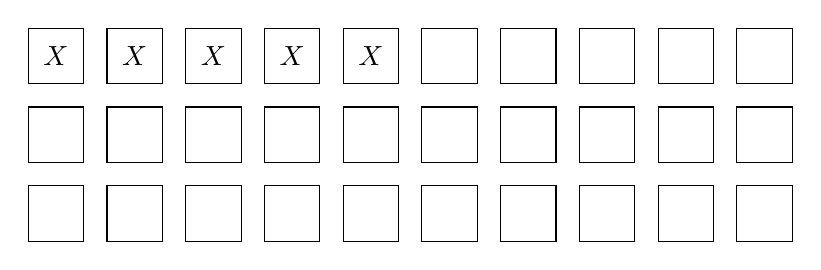
\begin{tikzpicture}
	%\node at (0,0) {$\checkmark$};
		 \foreach \x in {1,...,10}{
		\foreach \y in {0,...,2}{
       \node [inner sep=10pt, draw] at  (\x,\y)  {};
       }
			}
		\foreach \x in {1,..., 5}{
		\node [] at  (\x,2)  {\(X\)};
		}
	\end{tikzpicture}
		\end{center}
		
		\item Type ``number of ways to roll 4 dice with a sum \(<=\) 14 into \texttt{WolframAlpha.com}. Use this to calculate the probability of making the cut in 30 tournaments in a row. \label{tiger3}
		
	\end{enumerate}
		\item Based on Tiger Wood's golfing ability, the book shows that Tiger Woods gains, on average, more than two strokes per round. This is then used to decide that Tiger makes the cut when the four dice roll sums to 16 or less. Explain the reasoning behind this change. \vfill
		\item Based on Tiger Wood's consist play, the book reduces his standard deviation from 4 holes per round to 2 holes per round. They do this by assigning him a 68 for a two-dice sum of 7 and only adding one stroke for each number above and below 7.  Fill in the table again.
		
		\begin{center} \Large
		\begin{tabular}{c|c}
		Dice Roll & Round Score\\\hline
		4 & \\\hline
		5 & \\\hline
		6 & \\\hline
		7 & 68\\\hline
		8 & \\\hline
		9 & \\\hline
		10 & \\\hline
		\end{tabular}
	\end{center}\normalsize
\item If you take a four-dice roll of 18 or less to make the cut, what is Wood's probability of making the cut in 1 tournament? Explain using your work above why this dice cut-off for the cut based on your work above.
%You may want to use \texttt{WolframAlpha.com} again. What is the probability that he makes the cut in 30 tournaments in a row? Compare that with your answer to \ref{tiger3}. \vfill
\end{enumerate}
\stepcounter{chaptno}
\worksheet{Moneyball Analytics}

The Pythagorean expectation from the chapter says 
\[ P = \frac{RS^2}{RS^2+RA^2}\]
where $RS$ is runs scored, \(RA\) is runs allowed, and \(P\) is the percent of games the team is expected to have won. While the book says that the Pythagorean expectation is loosely connected to the Pythagorean Theorem, \(a^2+b^2=c^2\), \(P\) is more closely aligned to trig functions and could be considered the \(\sin^2(\theta)\) of the following triangle:

\begin{center}
	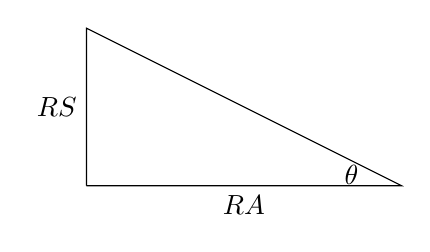
\begin{tikzpicture}
		\draw (0,0) -- node[below, pos=0.5] {\(RA\)} (4,0) node[shift={(-18pt,4pt)}] {\(\theta\)} -- (0,2) -- node[left, pos=0.5] {\(RS\)} (0,0);
	\end{tikzpicture}
\end{center}

\textbf{Worksheet: Compute Like Bill James}

\noindent Test James' Pythagorean expectation for another team. Pick a year and a Major League Baseball Team. Everyone gets a unique team/year.

\begin{enumerate}
	\item Find \emph{runs scored} by your team (RS): \underline{\hspace{2cm}}
	\item Find \emph{runs allowed} by your team (RA): \underline{\hspace{2cm}}
	\item Compute \( P = \frac{RS^2}{RS^2+RA^2}\): \underline{\hspace{2cm}}
	\item Compute \(P\times 162\): \underline{\hspace{2cm}}
\end{enumerate}
The result in line 4 is an estimate of how many games your team won in the season you chose. How close is it to the actual statistic? (For a year before 1962 or the short 2020 season, substitute the appropriate number of games.
\vfill
\clearpage

Baseball is a sport filled with statistics, but it is not the only one. Consider a sport other than Baseball that you follow. What statistics similar to \emph{runs for} and \emph{runs against} do you think would be  a good substitute in that sport? Try it for one team for one season for your sport.
\begin{enumerate}
	\item Find statistic \(S\) for your team: \underline{\hspace{2cm}}
	\item Find similar statistic for the other team \(OT\): \underline{\hspace{2cm}}
	\item Compute \( P = \frac{S^2}{S^2+OT^2}\): \underline{\hspace{2cm}}
	\item Compute \(P\times\) games played: \underline{\hspace{2cm}}
\end{enumerate}
How did you do? Is it as close as for baseball?
\vfill
Another thing that can be considered is the exponent in the Pythagorean expectation. In a more general world, you could change the exponent from 2 to \(a\) \footnote{This is taking us from the trigonometry of circles into a new world of the trigonometry of squircles. Come see me if you are curious.} and have a formula more like
\[ P = \frac{S^a}{S^a+OT^a}\]
Play around with different values of \(a\) to see if you can get a better estimate of the percent of games won.  What happens to the number as you increase \(a\) from 2 to something larger?  What would happen if you made \(a\) between 0 and 2?\vfill

\end{document}
